\begin{figure}[h]
\centering
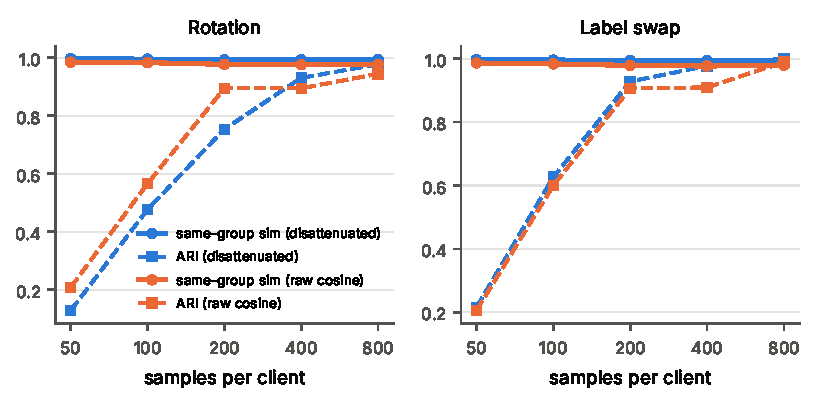
\includegraphics[width=0.85\linewidth]{../results/figures/sample_size.pdf}
\caption{Same-group similarity (solid) and ARI (dashed) as a function of the client size. Blue: disattenuated; orange: raw cosine.}\label{fig:size}
\end{figure}
\begin{figure}[h]
\centering
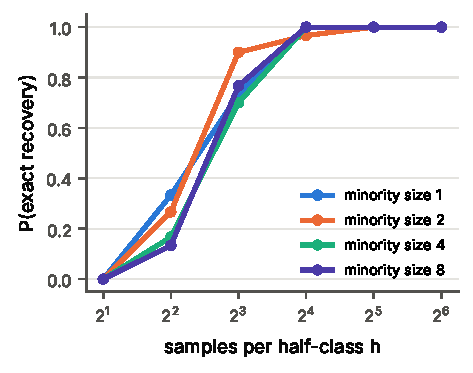
\includegraphics[width=0.45\linewidth]{../results/figures/theory_minority.pdf}
\caption{Synthetic validation of Corollary~\ref{cor:sc}: exact recovery of a minority group does not depend on its size.}\label{fig:thminority}
\end{figure}
\begin{table}[h]
\centering
\caption{Sensitivity to the shrinkage $\lambda$ at $\tau=0.9$: ARI / number of clusters (3 seeds, clustering step). For the label-only scenario the correct $K$ is 1. Only $\lambda=0.02$ and $0.1$ satisfy the condition of Corollary~\ref{cor:sc} when $\gamma=0.1$.}\label{tab:lambda}
\small
\begin{tabular}{lccccc}
\toprule
Scenario & $\lambda=0.02$ & $\lambda=0.1$ & $\lambda=0.2$ & $\lambda=0.5$ & $\lambda=1.0$ \\
\midrule
Rotation & 0.93 / 4.3 & 0.93 / 4.3 & 0.93 / 4.3 & 0.93 / 4.3 & 0.93 / 4.0 \\
Label swap & 0.98 / 4.0 & 0.98 / 4.0 & 0.98 / 4.0 & 0.98 / 4.0 & 0.98 / 4.0 \\
Rotation + QS & 0.92 / 5.0 & 0.92 / 5.0 & 0.91 / 5.0 & 0.98 / 4.3 & 0.98 / 4.0 \\
Mixed + QS & 0.96 / 4.0 & 0.96 / 4.0 & 0.96 / 4.0 & 0.96 / 4.0 & 0.96 / 4.0 \\
Label skew only & 1.00 / 1.0 & 1.00 / 1.0 & 1.00 / 1.0 & 1.00 / 1.0 & 1.00 / 1.0 \\
Minority groups & 1.00 / 4.0 & 0.99 / 4.3 & 0.99 / 4.3 & 0.99 / 4.0 & 1.00 / 4.0 \\
\bottomrule
\end{tabular}
\end{table}


\begin{table}[!htbp]
\centering
\caption{Hierarchical comparison of DisCo-CFL with each baseline on the held-out runs only, i.e.\ excluding the development runs listed in Section~\ref{sec:setup}. Columns as in Table~\ref{tab:hier}.}\label{tab:hier_heldout}
{\scriptsize
\begin{tabular}{l c c c c c c c c c}
\toprule
Baseline & \multicolumn{3}{c}{Accuracy} & \multicolumn{3}{c}{Concept acc.} & \multicolumn{3}{c}{Worst group} \\
\cmidrule(lr){2-4}
\cmidrule(lr){5-7}
\cmidrule(lr){8-10}
 & $\Delta$ [95\% CI] & W/T/L & p & $\Delta$ [95\% CI] & W/T/L & p & $\Delta$ [95\% CI] & W/T/L & p \\
\midrule
\multicolumn{10}{l}{\textit{(a) Small-CNN benchmarks (main, other, sweep scenarios pooled)}} \\
FedAvg & +6.7 [+4.6, +9.0] & 16/3/0 & <0.001 & +11.7 [+8.1, +15.5] & 16/2/1 & <0.001 & +10.0 [+6.3, +14.2] & 16/2/1 & <0.001 \\
Local & +0.6 [$-$1.9, +2.5] & 9/0/2 & 0.160 & +20.5 [+15.9, +24.9] & 11/0/0 & <0.001 & +0.3 [$-$2.8, +2.9] & 9/0/2 & 0.160 \\
FedAvg-FT & +2.6 [+0.2, +4.5] & 9/0/2 & 0.034 & +8.7 [+6.4, +10.5] & 10/0/1 & <0.001 & +3.3 [$-$0.1, +6.0] & 9/0/2 & 0.034 \\
IFCA & +1.6 [+0.2, +2.8] & 16/1/2 & 0.010 & +7.3 [+4.7, +9.9] & 17/0/2 & <0.001 & +2.4 [+0.6, +4.0] & 17/0/2 & 0.005 \\
FeSEM & +2.9 [+1.6, +4.1] & 16/0/3 & <0.001 & +9.3 [+7.2, +11.5] & 19/0/0 & <0.001 & +4.7 [+2.8, +6.6] & 17/0/2 & <0.001 \\
MTCFL & +0.9 [$-$0.6, +2.1] & 17/0/2 & 0.007 & +12.0 [+10.7, +13.2] & 19/0/0 & <0.001 & +0.8 [$-$1.1, +2.4] & 17/0/2 & 0.009 \\
FL+HC & +1.1 [+0.3, +1.9] & 15/1/3 & 0.005 & +4.7 [+3.4, +6.1] & 18/0/1 & <0.001 & +1.4 [+0.2, +2.6] & 15/1/3 & 0.011 \\
PACFL & +3.7 [+0.9, +6.7] & 15/1/3 & 0.004 & +9.2 [+4.3, +14.4] & 17/0/2 & <0.001 & +5.7 [+1.9, +10.2] & 16/0/3 & 0.002 \\
StoCFL & +4.3 [+2.4, +6.1] & 17/0/2 & <0.001 & +14.8 [+11.6, +18.0] & 19/0/0 & <0.001 & +6.0 [+3.1, +9.2] & 17/0/2 & <0.001 \\
StoCFL-W & +2.1 [+0.8, +3.2] & 16/0/3 & 0.004 & +10.5 [+8.7, +12.3] & 19/0/0 & <0.001 & +2.5 [+0.8, +4.0] & 16/0/3 & 0.005 \\
FedCCFA & +2.8 [+0.9, +4.3] & 17/0/2 & 0.001 & +10.3 [+8.1, +12.2] & 18/0/1 & <0.001 & +4.0 [+1.3, +6.3] & 17/0/2 & <0.001 \\
FedDAG-C & +2.0 [+0.7, +3.3] & 15/0/4 & 0.003 & +7.5 [+4.8, +10.5] & 19/0/0 & <0.001 & +3.2 [+1.3, +5.2] & 15/1/3 & 0.001 \\
\addlinespace
\multicolumn{10}{l}{\textit{(b) Realistic benchmarks}} \\
FedAvg & +1.4 [$-$0.3, +3.0] & 4/0/1 & 0.094 & +2.0 [$-$0.6, +4.4] & 3/0/2 & 0.156 & +1.5 [$-$1.1, +4.0] & 3/0/2 & 0.156 \\
Local & +9.4 [+5.3, +13.5] & 5/0/0 & 0.031 & +31.1 [+28.1, +33.8] & 5/0/0 & 0.031 & +9.7 [+5.8, +13.7] & 5/0/0 & 0.031 \\
FedAvg-FT & +6.9 [+4.6, +9.9] & 5/0/0 & 0.031 & +7.3 [+3.5, +11.2] & 5/0/0 & 0.031 & +9.4 [+3.7, +15.9] & 5/0/0 & 0.031 \\
IFCA & +3.6 [+2.0, +5.9] & 5/0/0 & 0.031 & +7.7 [+5.7, +9.8] & 5/0/0 & 0.031 & +3.8 [+1.0, +6.6] & 4/0/1 & 0.062 \\
FeSEM & +2.6 [+1.4, +4.1] & 5/0/0 & 0.031 & +5.4 [+3.3, +7.4] & 5/0/0 & 0.031 & +2.9 [+0.5, +5.2] & 4/0/1 & 0.062 \\
MTCFL & +3.7 [+1.8, +5.7] & 5/0/0 & 0.031 & +14.1 [+12.7, +15.4] & 5/0/0 & 0.031 & +3.8 [+1.2, +6.2] & 5/0/0 & 0.031 \\
FL+HC & +1.5 [+0.3, +2.5] & 4/0/1 & 0.062 & +3.6 [+0.4, +6.7] & 4/0/1 & 0.062 & +2.5 [+0.6, +4.7] & 5/0/0 & 0.031 \\
PACFL & +1.9 [+0.2, +4.2] & 4/0/1 & 0.094 & +3.9 [+1.4, +6.4] & 4/1/0 & 0.062 & +1.7 [$-$1.5, +4.9] & 4/0/1 & 0.219 \\
StoCFL & +3.2 [+0.9, +5.4] & 4/0/1 & 0.062 & +12.7 [+3.5, +22.7] & 4/0/1 & 0.062 & +3.4 [+1.2, +5.5] & 4/0/1 & 0.062 \\
StoCFL-W & +4.8 [+2.3, +7.4] & 5/0/0 & 0.031 & +17.4 [+12.5, +22.4] & 5/0/0 & 0.031 & +4.8 [+1.4, +8.1] & 5/0/0 & 0.031 \\
FedCCFA & +2.4 [+1.8, +3.1] & 5/0/0 & 0.031 & +4.1 [+1.5, +6.7] & 5/0/0 & 0.031 & +3.0 [+1.3, +4.3] & 5/0/0 & 0.031 \\
FedDAG-C & +3.0 [+1.6, +4.7] & 5/0/0 & 0.031 & +7.5 [+4.3, +11.0] & 5/0/0 & 0.031 & +3.9 [+1.9, +6.3] & 5/0/0 & 0.031 \\
\bottomrule
\end{tabular}
}

\end{table}
